\section{Neural Networks}
\label{sec:nn}

Inspired by biological nervous systems, such as the human brain, artificial neural networks are used for information processing. In biological nervous systems, highly interconnected neurons work together to solve a specific task\cite{ArtNNKapil}. Each neuron solves a subtask and communicates with other neurons. In artificial neural networks this idea is used to approximate arbitrary  non-linear functions. The nodes (neurons) are connected by weighted edges and the topology is chosen depending on the problem. In the training phase, the weights of the edges are set depending on the data. Neural networks are often represented in layers - each layer contains some of the nodes and then follows the interconnections to the next layer. These connections add high flexibility and the potential to self-organize.

The power of neural networks lies in its ability to learn and generalize \cite{Haykin:1998:NNC:521706}. That means that even for data not encountered during training, the network produces reasonable outputs. 

\subsection{Compression with Neural Networks}
Most compression algorithms that use neural networks fall into one of three categories\cite{Dony1995}: 

\subsubsection{Predictive Coding}
Predictive coding aims to reduce redundancies by decorrelating the data. An estimate \(\hat{x}(n)\) is calculated by applying a predictor to the current pixel and neighboring pixels, i.e. by
\begin{equation}
\hat{x}_n = \sum_{j=1}^{p} w_j x(n-j)
\end{equation}
where \({w_j}\) is a set of coefficients from a statistical model called autoregressive model. The mean squared error is then minimized by satisfying \(Rw = d\), where \(R_{ij}\) is the \emph{ij}-th element of the autocovariance matrix and \(d_j = E[\hat{x}(n)x(j)]\).

\subsubsection{Transform coding}
In transform coding, one chooses a transformation that produces a set of coefficients such that a subset of these coefficients is sufficient to reconstruct the original data. One such transform coding is linear block transform coding, a technique that uses orthonormal basis vectors \(w_i\) in the transformation matrix \(W\). The output vector \(y = Wx\) is the coefficient vector of \(x\), a length \(N = n^2\) vector of an \(n \times n\) image block. The vectorized image is then given as \(\hat{x} = W^Ty\). 
A famous example for linear block transform coding is the image compression standard JPEG.

\subsubsection{Vector quantization}
This approach maps a block of the original input data, based on some distance metric, to one of several codewords. It exploits the correlation between neighboring pixels. To reconstruct the data, only the index of the codeword in the codebook is needed. 

\subsection{Direct classification}
In \cite{Soliman2006258}, the authors use adaptive vector quantization, together with an universal codebook, to divide the subimages into clusters. Their \emph{direct classification} approach combines the two neural networks models Kohonen and ART1, exploiting the reliability of the first and the speed of the second model. By using an universal codebook, they are able to increase the compression ratio significantly, though the image quality decreases.

\subsection{Neural Network Structure} \label{sec:neural_net_structure}
\begin{figure}[tbp]
  \centering
  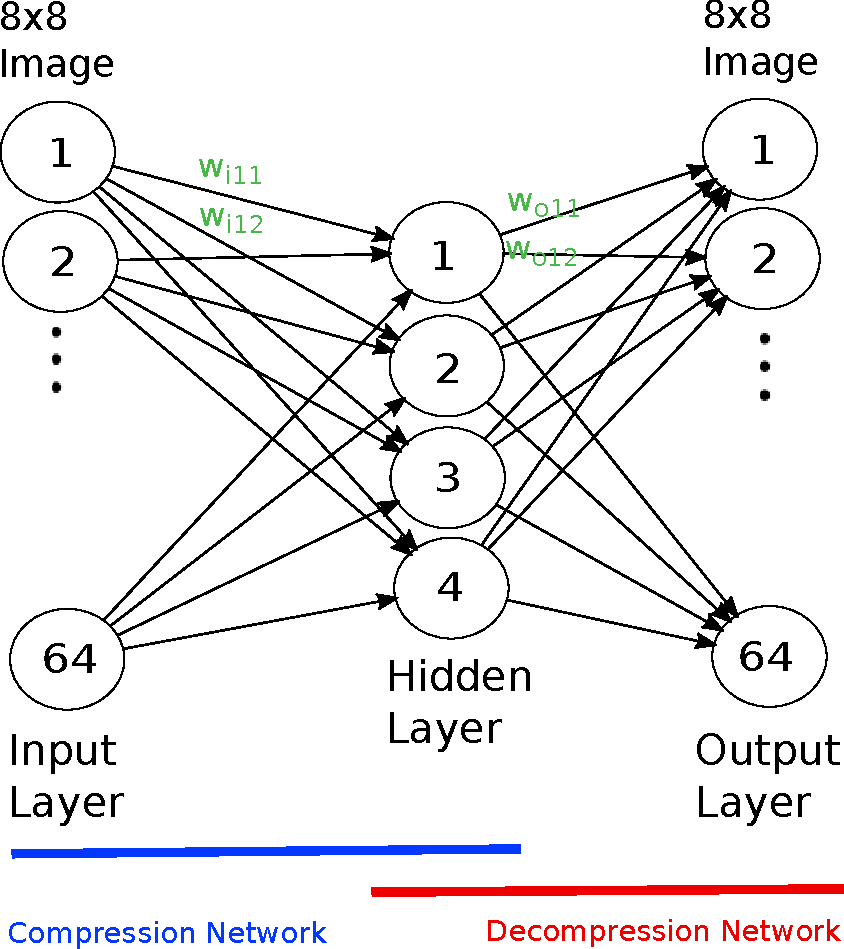
\includegraphics[width=0.33\textwidth]{images/nnStructure}
  \caption{Neural Network Structure.}
  \label{fig:nnStructure}
\end{figure}

Figure~\ref{fig:nnStructure} shows the neural network structure we use for compression. There are three types of layers: input layer, hidden layer and output layer. The input layer and the hidden layer are fully interconnected, as are the hidden layer and the output layer. The weights of the edges are determined by the training algorithm that is described in section~\ref{sec:trainfcn}. This kind of neural network is also called bottleneck-like neural network, because the hidden layer is a bottleneck.

